\vspace{-3mm}
\section{Evaluation}

We tested our prototype of DASF on a Galaxy Nexus (\textit{GT-I9250}),
which includes a 1.2 GHz dual-core ARM Cortex-A9 processor,
1 GB of RAM, and 16 GB of flash memory.  Our goal is to
illustrate that DASF provides adequate protection against the
previously discussed security threats and provides a reasonable
performance overhead.

\subsection{Security Threat Evaluation}

As previously discussed, we consider four different types of security
threats that DASF must provide protections against
\textit{(1) legitimate user misbehavior},
\textit{(2) malicious users}, \textit{(3) application misbehavior},
and \textit{(4) malicious applications}.  Since CleanOS addresses
the 2nd security threat by providing a mechanism for revoking sensitive
data and we assumed that our model was built on top of CleanOS, we do not
evaluate that security threat.  However, we perform the following three
tests to show that DASF adequately addresses the remaining
security threats.

\begin{itemize}
\item \textit{Legitimate user misbehavior.}  We created an application that receives
  data from the server that has restrictions imposed on the data.  Next, we
  attempt to manually save and forward the data by passing it to other
  applications on the device that attempt to perform these operations.
\item \textit{Application misbehavior.}  We created an application that requests
  data from the server (e.g., an MRI image) that is restricted to be saved
  to the device.  When the application is receiving the data, it attempts
  to break the policy by writing the data directly to a file when receiving
  it.
\item \textit{Malicious applications.}  We created a malicious voice memo recorder
  application that attempts to steal information from the environment. Our
  voice memo recorder requests the \textit{record audio} permission
  and the \textit{internet} permission to allow users to sync memos to their
  other devices.  However, the voice memo recorder maliciously launches
  a background service to secretly record audio in the background and
  transmits the recorded audio to an external server.
\end{itemize}

We ran the first test and confirmed that DASF successfully
blocked the data from being forwarded from the device and saved to the device.
Thus, DASF enforced the policy imposed on the data from the
server.

When we ran the second test, we confirmed that DASF
successfully blocked the data from being saved to a file.  Moreover, we
modified the application to check the sensitivity level on the data
received and determine whether to store the data in a file or keep it
in main memory.

Finally, we ran the third test by starting the malicious
voice memo recorder and confirmed that it successfully recorded data in the
background.  Next, we created another application that restricts the
\textit{record audio} permission when the user presses a button.  DASF
successfully closed the malicious voice memo recorder, including its
background service, and prevented it from being opened again until
the \textit{record audio} permission was unrestricted.  Instead of
restricting the permission by pressing a button, an application can
be designed to restrict permissions when certain RFID tags are
scanned, which would allow doctors to simply wave their device by
an RFID tag when entering areas where conversations may include
PHI data (e.g., outside of patient rooms).  To prevent malicious
applications from attempting to steal sensitive information stored on
the device (e.g., PHI information authorized to be saved to the device),
we rely on Android's file system privileges (e.g., UIDs) and our restriction
that medical applications are assigned a unique UID.  

\vspace{-3mm}
\subsection{Performance Evaluation}

Since DASF is invoked whenever an application, or application
component is started, we tested the performance overhead on the starting
activities and services on the Galaxy Nexus running our prototype.  To get
a baseline for comparison, we repeated the tests on the stock Android \textit{Jelly Bean}
platform and on TaintDroid.  Furthermore, we also tested the overhead of
\textit{medical applications} using our message protocol.

\textbf{Application Component Overhead.}  Whenever an activity or service is
started, our\textit{Privilege Restriction Service} is invoked to determine
whether the activity or service may be started.  Therefore, we tested
the time that it takes to launch activities and service.  We repeated
the same tests on the stock Android \textit{Jelly Bean} platform and on TaintDroid.

Fig.~\ref{fig:component} shows the performance overhead of starting activities and services on
our prototype, the stock Android \textit{Jelly Bean} platform, and on TaintDroid.
As the figure shows, our prototype took 118 milliseconds on average to
start an activity and 17 milliseconds on average to start a service.  The
stock Android \textit{Jelly Bean} platform took 94 milliseconds on average
to start an activity and 8 milliseconds on average to start a service.  The
TaintDroid platform took 115 milliseconds on average to start an activity
and 14 milliseconds on average to start a service.  We assume that the
overhead when comparing TaintDroid and the stock Android \textit{Jelly Bean}
platform is due to the extra memory that needs to be allocated for the 
taint tags in the Java stack.  When compared to the overhead of TaintDroid,
using our prototype results in a minimal overhead on starting activities and services.

\begin{figure}[ht]
\centering
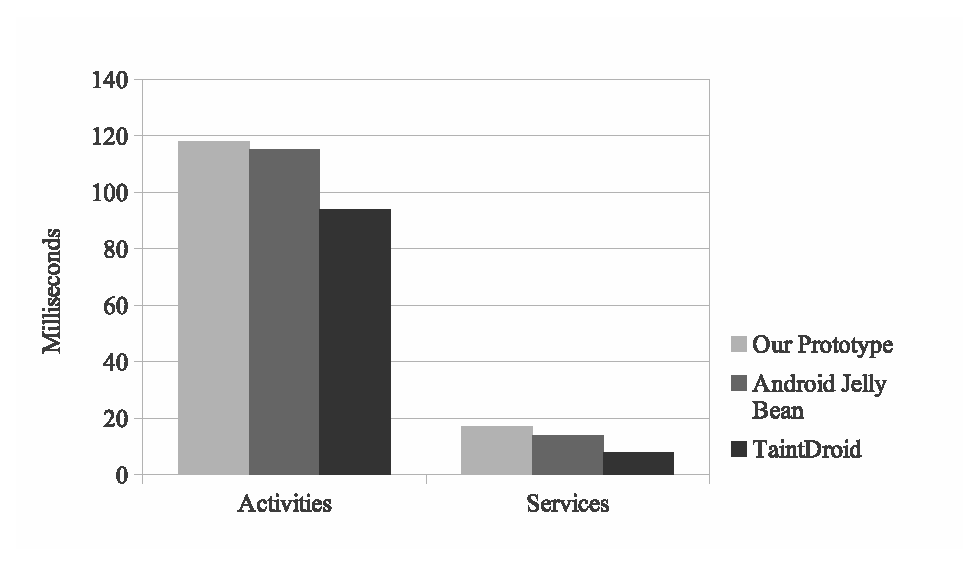
\psfig{file=component_performance.eps, width=2.6in}
\caption{Performance overhead when starting activities and services}
\label{fig:component}
\end{figure}

\textbf{Message Protocol Overhead.}  To test the overhead of our message protocol,
we created an application that requested data of varying length from the server.
The data lengths that we tested are 1-KB, 5-KB, 100-KB, 1-MB, 5-MB, and 50-MB.
We have recorded the time that it took the \textit{MessageInputStream} to receive
the message and pass the data back to the application.  We disregarded the time
that it took to transmit the data over the network since that is related
to the overhead of the network speed rather than the overhead caused by
our message protocol.  Furthermore, we also recorded the time that it
took the system to enforce policy restrictions and unrestrictions.

As the Fig.~\ref{fig:performance} suggests, our message
protocol took 54931 nanoseconds on average to parse and return 1-KB of
data back to the application, 73242 nanoseconds on average for 5-KB, 
720215 nanoseconds on average for 100-KB, 8 milliseconds on average
for 1-MB, 49 milliseconds on average for 5-MB, and 468 milliseconds
on average for 50-MB.  Furthermore, it took 81 milliseconds on average
to impose permission restrictions and around 2 milliseconds on average
for permission unrestrictions.

\begin{figure}[ht]
\centering
\subfigure[Data Message Overhead]{
	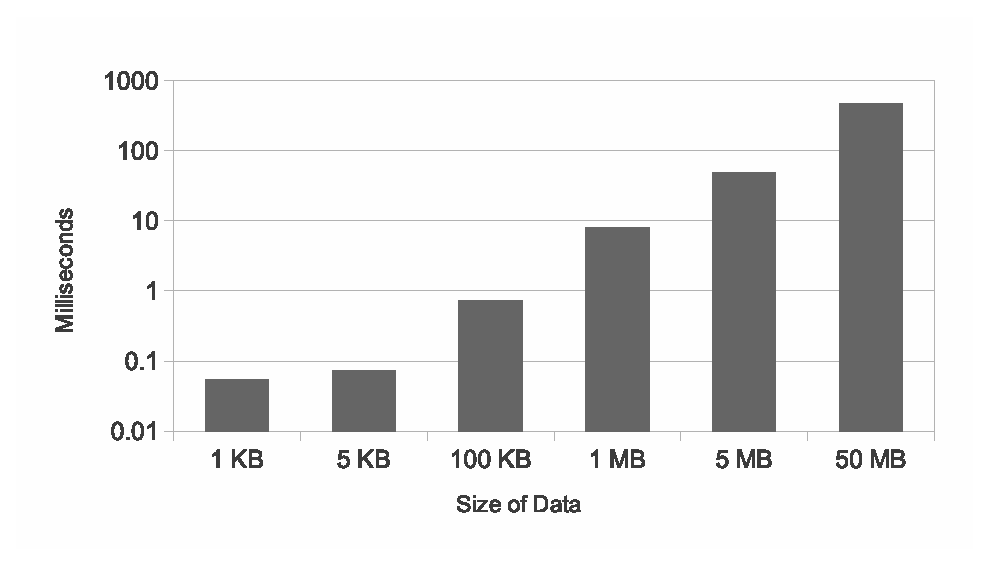
\psfig{file=kb_performance.eps, width=2.6in}
	\label{fig:kbperformance}
}
\subfigure[Privilege Control Message Overhead]{
	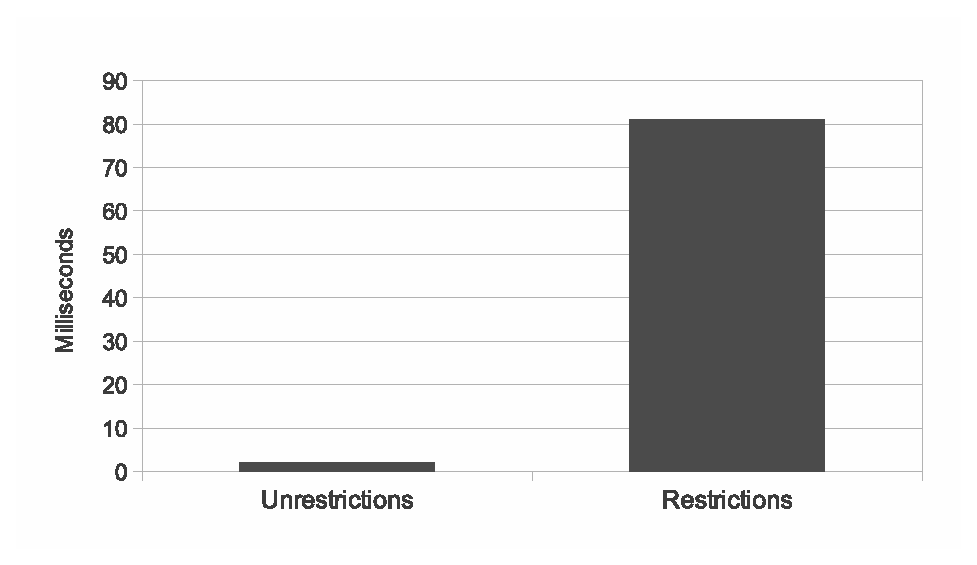
\psfig{file=policy_performance.eps, width=2.4in}
	\label{fig:policyperformance}
}
\caption{Message Protocol Performance Overhead}
\label{fig:performance}
\end{figure}

\subsection{Limitations}

There are three current limitations of the DASF prototype.  First,
the sensitivity level of the data can be cleared since TaintDroid's
taint propagation logic does not address implicit flows. This is a major
concern because applications can clear the sensitivity
level from data and break the security policies imposed on that data.
Second, TaintDroid also does not allow applications to use third-party
native libraries since they can be used to clear privacy tags.  Third,
DASF does not currently handle propagating
the sensitivity level of data displayed on the screen.  Therefore,
a user can break the security policy on sensitive data by taking a
screenshot of an image.

